\documentclass{article}
\usepackage[T1]{fontenc}

\def \figwidth{0.8\textwidth}

%% The packages beton, concmath, and ccfonts are LaTeX packages that
%% change the default text fonts from Computer Modern to
%% Concrete. Packages beton and ccfonts also slightly increase the
%% default value of \baselineskip to account for the rather heavier
%% weight of the Concrete fonts.
\usepackage{beton}
\usepackage{concmath}
\usepackage{ccfonts}
\usepackage{eulervm}

\usepackage{graphicx}
\usepackage{listings}
\usepackage{float}
\usepackage[margin=2.5cm]{geometry}
\usepackage{verbatim}
\usepackage{subfigure}
\usepackage{wrapfig}
\usepackage{url}

\title{Coarse Grained Parallelism in VTK}
\date{}
\begin{document}
\maketitle{}

The goal of this article is to answer the question: Should we adopt
more coarse grained multithreading in VTK? In order to understand the
potential benefits and work involved, we implement a few new coarse
grained multithreading features for VTK execution pipeline.

For all experiments, we use the machine kadoop1 at KRS. This machine
has two quad-core processors---making up a total of eight cores.

\subsubsection*{Code References}
\begin{itemize}
\item Changes to VTK code can be checked out from the branch
  parallel-composite-pipeline in
  \url{git://github.com/leo1978/berks-vtk.git}.  If you do not want to
  use some experimental performance enhancement code, you can also
  check out the topic "Towards a generic multithreading framework'' from the branch.
\item Test program code can be found at the master branch of
  \url{git://github.com/leo1978/tbb.git}. There is a python script
  ``./testall.py'' that tests the most important programs.
\end{itemize}


\section{Intel TBB library}
We rely on the Intel library Thread Building Block (TBB) for thread
management. The reason for using such an external library is that
wider adaptation of multithreading will almost certainly require some
type of thread pool and dynamic load balancing, which VTK does not
currently provide.

The main benefit of using thread pool is that the overhead of creating
and destroying threads is minimized. In our experience, during a
single program run, TBB never creates more threads than what is
necessary to achieve the maximum parallelism, e.g. four threads on a
quad-core machine. In contrast, {\tt vtkMultiThreader} will create as many
threads as tasks.

TBB performs load balancing automatically. To test whether the
automatic load balancing works as advertised, we create a simple
test, where a single ``unbalance'' parameter $k$ controls how a
fixed amount of work $w$ is distributed among a set of $n$ tasks: For
task $0\le i<n$, its work is
$w\left(k(\frac{2i}{n}-1)+\frac{1}{n}\right)$.

Figure~\ref{fig:unbalance} shows that TBB load balancing performs
well, resulting almost constant running time, while not load balancing
results in running time that degrades with the unbalance parameter.
\begin{figure}[H]
\centering{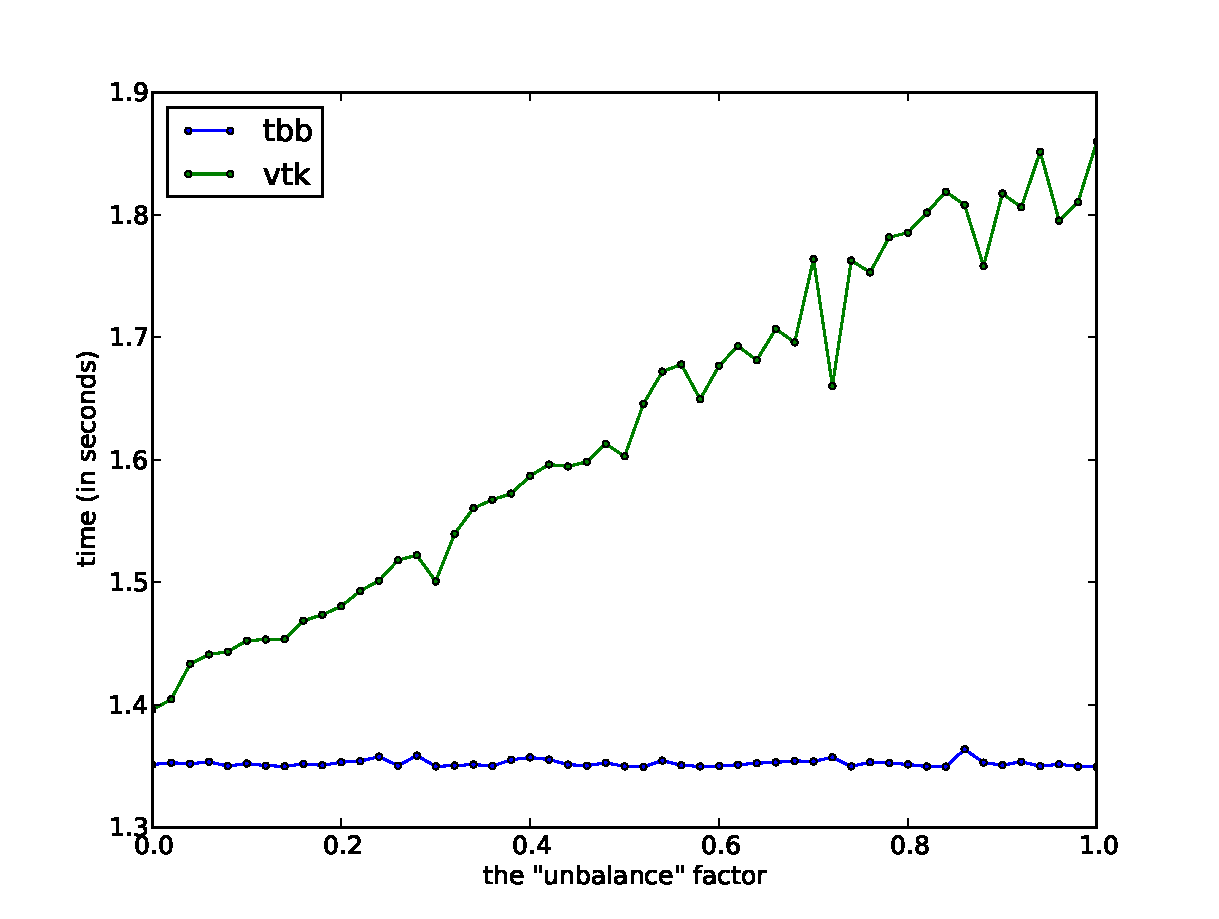
\includegraphics[width=0.6\textwidth]{unbalance.pdf}}
\caption{Running time as a function of the ``unbalance'' factor.  Each
  data measurement is averaged over 10 runs. The ``tbb'' plot gives
  the result using {\tt tbb::parallel\_for}, and the ``vtk'' plot
  gives the results by first partitioning the tasks evenly in indices
  and running the threads using \texttt{vtkMultiThreader}}
\label{fig:unbalance}
\end{figure}

\subsubsection*{Code References}
\begin{itemize}
\item Build configuration: Debug.
\item Run {\tt ./testparallelfor [balance factor between 0 and 1]
  [-vtk|-tbb|-1]}, where the option ``-vtk'' uses vtkParallelFor and
  ``-1'' means single threaded execution.
\item To generate the plots, run {\tt python ./analyze-vtk-tbb.py [output without -noTbb] [output with -noTbb]}.
\end{itemize}


\section{Testing correctness using {\tt vtkParallelFor}}

One drawback of using TBB is that it does not work well with
helgrind---a popular open source tool for detecting race
conditions. Running helgrind on TBB code generates many false positives
even for extremely simple codes, and it is not clear how the false
positives can be suppressed correctly.


For the purpose of correctness check, and also for comparing
performance against a naive multithreading scheme, we implemented a
template algorithm {\tt vtkParallelFor} on top of existing VTK
threads that have the same input and output as {\tt
  tbb::parallel\_for}, so switching between the two is easy.

\section{Multithreaded Composite Data Executive}

The current composite data pipeline iterates through the data blocks
in a composite data and executes the algorithm for each block. We
replace the serial execution by parallel execution. For each parallel
task, we construct input and output vtkInformation objects before
passing them to the filter. The code changes involves a small amount
of refactoring of the class {\tt vtkCompositeDataPipeline} for the purpose
of introducing a multithreaded child {\tt vtkThreadedCompositeDataPipeline},
which handles all the multithreading work.

\subsection{Contouring AMR}
For this experiment, we form a processing pipeline with three
filters:

{\tt vtkAMRFlashReader}  $\rightarrow$ {\tt vtkCellDataToPointData}
 $\rightarrow$ {\tt vtkSynchronizedTemplates3D}.

The input is an AMR flash data set consists of 20K blocks of image
data. The output is approximately 1M polygons. We only time the
processing time of the last two filters, since only their times are
affected by multithreading. We use {\tt vtkParallelFor} for
comparison.

The running time from both the Release and Debug builds are shown in
the figure~\ref{fig:flash}. We suspect that the difference in scaling
behavior is due to the fact that individual images are very small (142
pixels on average). This causes the total running time to be sensitive
to the overhead per image.

We can also see that the performance of TBB is very similar to
vtkParallelFor. This can be read in two ways:
\begin{itemize}
\item The work load happens to be pretty evenly distributed across the
  AMR blocks so that TBB's load balancing cannot help much here.
\item TBB did a good job choosing big enough task sizes so that the
  overhead per task (constructing vtkInformation objects) becomes
  neglible after amotizing over all the blocks. We found that, in the
  quad core case, TBB created only 354 tasks in total, which implies
  an average task size of 54. Had we forced the task size to be 1, the
  processing time would have tripled.
\end{itemize}

\begin{figure}[H]
\centering \mbox{
  \subfigure{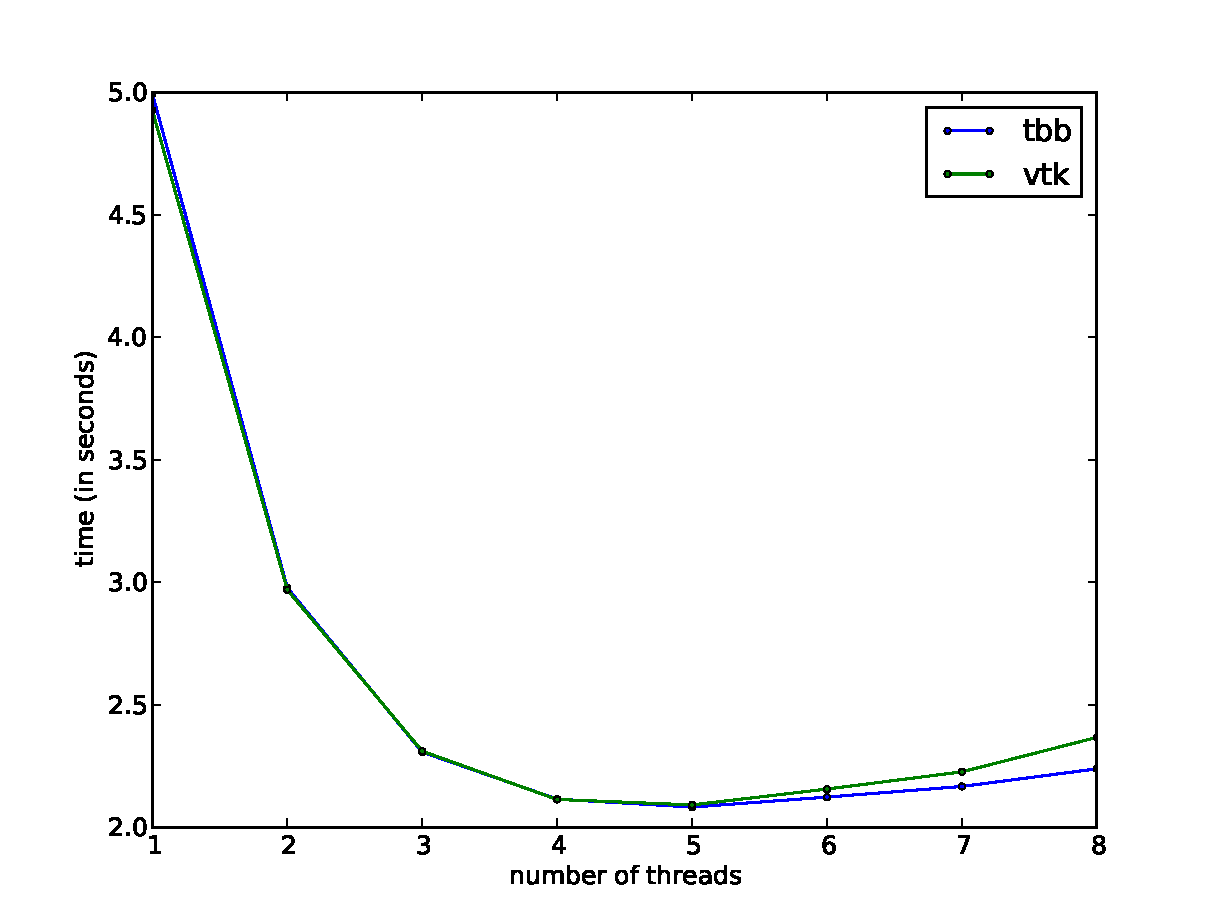
\includegraphics[width=0.5\textwidth]{contouramr.pdf}}
  \quad \subfigure{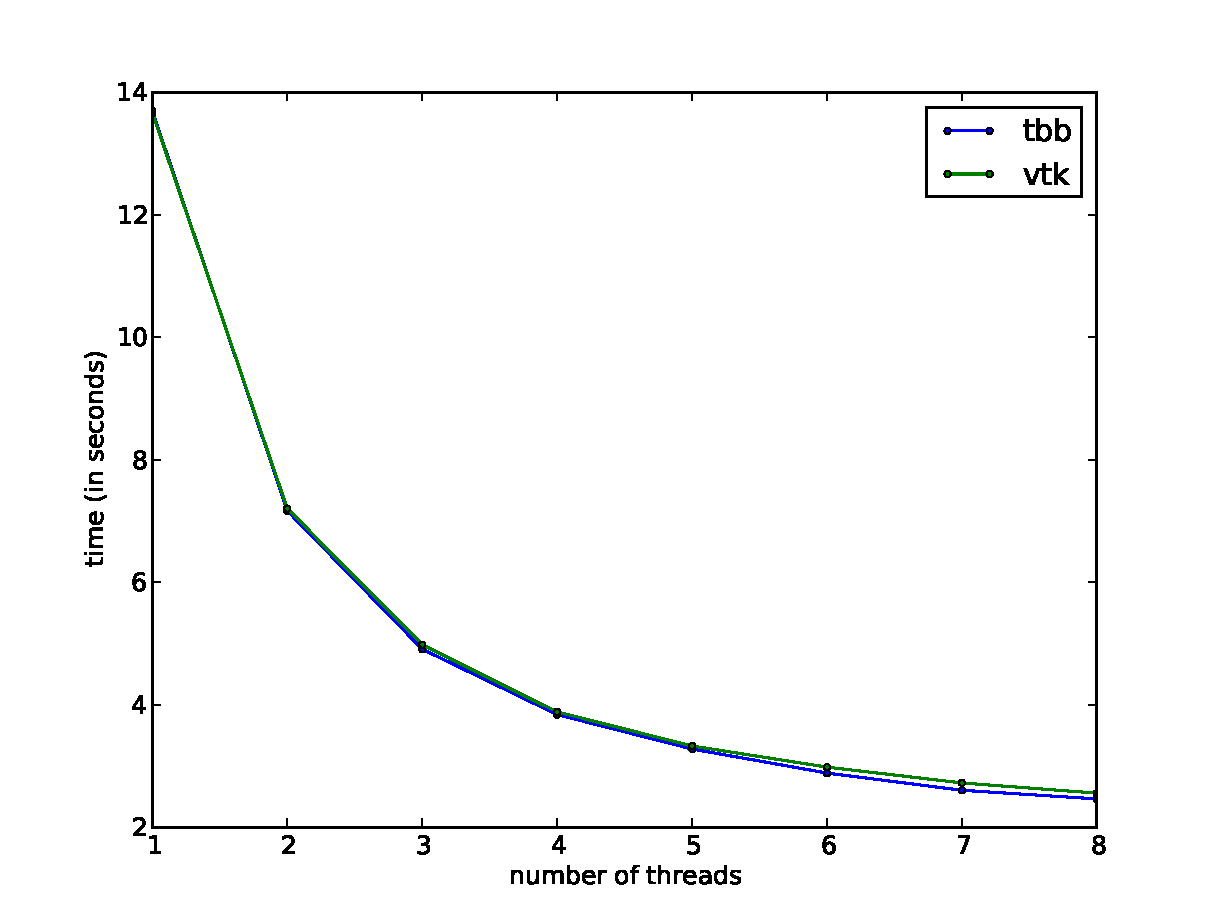
\includegraphics[width=0.5\textwidth]{contouramr-debug.pdf}}
}
\caption{Running time as a function of the number of parallel
  threads. Left: Release; Right: Debug. Each data measurement is
  averaged over 10 runs. The ``tbb'' plot gives the result using {\tt
    tbb::parallel\_for}, and the ``vtk'' plot gives the results by
  using {\tt vtkParallelFor}. }
\label{fig:flash}
\end{figure}

\subsubsection*{Code References}
\begin{itemize}
\item Build configuration: {\tt Release and Debug}.
\item To generate the plots, run
\begin{itemize}
\item {\tt python run.py "./contouramr -bigdata" > pcontour-tbb.log}
\item {\tt python run.py "./contouramr -bigdata -noTbb" > pcontour-vtk.log}
\item  {\tt python ./analyze-vtk-tbb.py pcontour-tbb.log pcontour-vtk.log}.
\end{itemize}

\end{itemize}

% sanity notes to self: should take about 5-seconds in serial release mode and 14 seconds in Debug mode

\subsection{Stream tracing}
For this experiment, we have a pipeline:

{\tt vtkRTAnalyticSource}  $\rightarrow$ {\tt vtkImageGradient}
 $\rightarrow$ {\tt vtkStreamTracer}.

The input is is an image of size $[-10,\ldots,10]^3$, together with
1000 seeds uniformly sampled on a plane. The output has 2.6M points.

We made the following code changes:
\begin{itemize}
\item The input seed points are created as a multiblock data set,
  where each block is a {\tt vtkPolyData} object with one point.
\item The output traces are merged after running the stream tracer using
{\tt vtkAppendPolyData}.
\item Refactoring out the member variables {\tt InputData}, {\tt
  HasMatchingPointAttributes}, and {\tt LastStepSize}.
\item In {\tt vtkStreamTracer}, replace call to {\tt vtkIdType*
  vtkImageData::GetIncrements()} by {\tt
  vtkImageData::GetIncrements(vtkIdType*)}.
\end{itemize}

\begin{figure}[H]
\centering{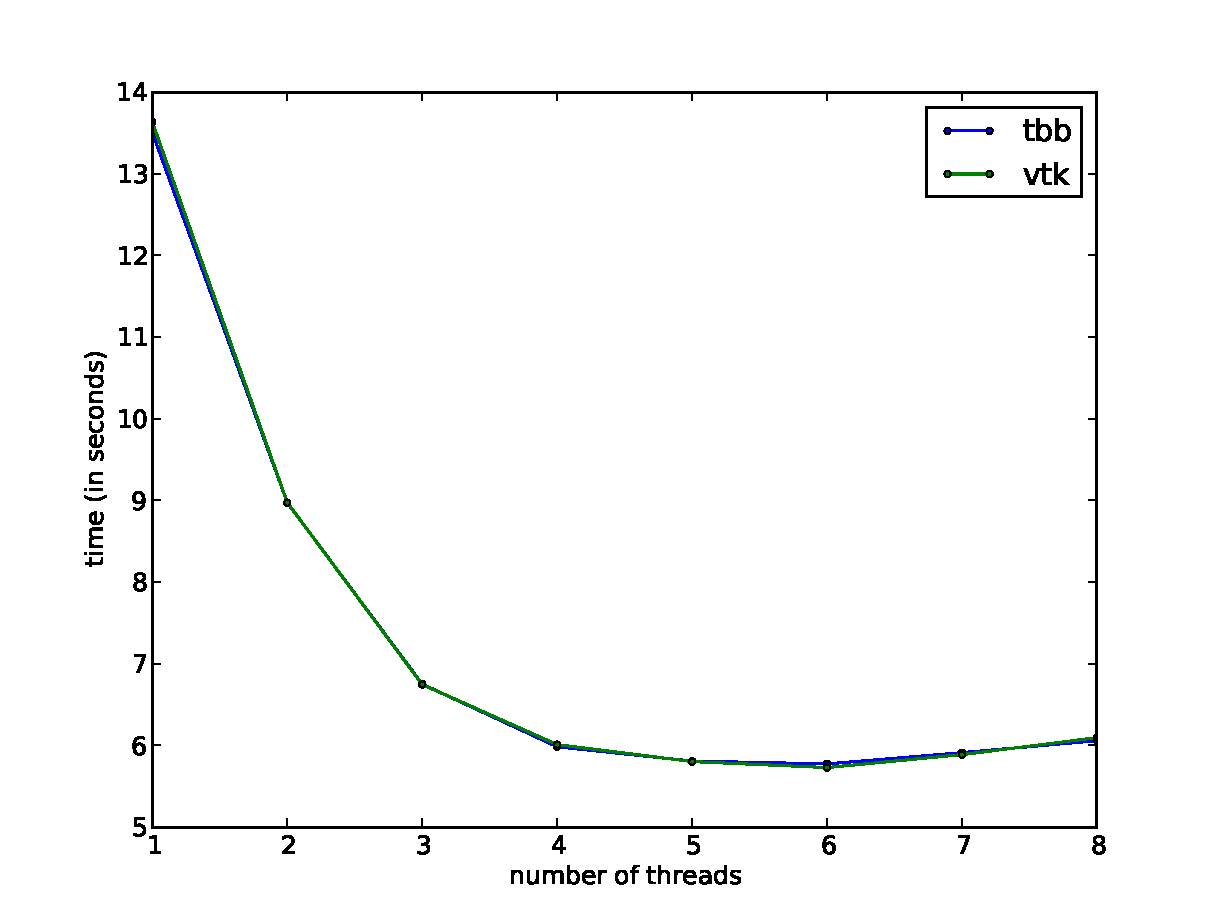
\includegraphics[width=0.6\textwidth]{stream-trace.pdf}}
\caption{Running time of stream tracing as a function of the number of parallel
  threads. Each data measurement is averaged over 10 runs. The
  ``tbb'' plot gives the result using {\tt tbb::parallel\_for}, and the ``vtk''
  plot gives the results by using {\tt vtkParallelFor} }
\label{fig:streamtrace}
\end{figure}

The running times are shown in
figure~\ref{fig:streamtrace}. Surprisingly, even with what seems to be
significant overhead of initializing the stream tracer, the running
time decreases nicely as the number of threads increases.

\subsubsection*{Code References}
\begin{itemize}
\item Build configuration: Release.
\item To generate the plots, run
\begin{enumerate}
\item {\tt python run.py "./threaded\_streamtrace -extent 100 -numTraces 1000" > stream-trace-tbb.log}
\item {\tt python run.py "./threaded\_streamtrace -extent 100 -numTraces 1000 -noTbb" > stream-trace-vtk.log}
\item {\tt python ./analyze-vtk-tbb.py stream-trace-vtk.log stream-trace-tbb.log}.
\end{enumerate}
\end{itemize}

\subsection{Contouring and Cutting Images }

We multithreaded two algorithms for contouring and cutting:
vtkSynchronizedTemplates3D and vtkSynchronizedTemplates3DCutter. These
algorithms already take input image extents, so we divide the tasks
according to image extents. The input is an image of size
$[-200,200]^3$, which we divide into $4^3=64$ chunks. Contouring
produces 1.3M points and 2.7M cells; cutting produces 0.12M points and
0.24M cells.

The most significant part of the work went in speeding up merging the
output from the chunks. The initial naive solution is to use
vtkAppendPolyData to union the output and then use vtkCleanPolyData to
resolve the duplicate points, but this turns out to be way too slow,
as vtkCleanPolyData spends more time than contouring. We are able to
implement a new algorithm that integrate functionality of both filters
but runs 20 times faster. This makes it feasible to take the
multithreaded approach.

In figure~\ref{fig:contour}, we can see that the running time scales
well, although merging time is still significant, particularly for
large number of threads. However, it does have the nice property of
being ``output sensitive'': this overhead directly depends on the
output size, rather than the input.

\begin{figure}[H]
\centering \mbox{
  \subfigure{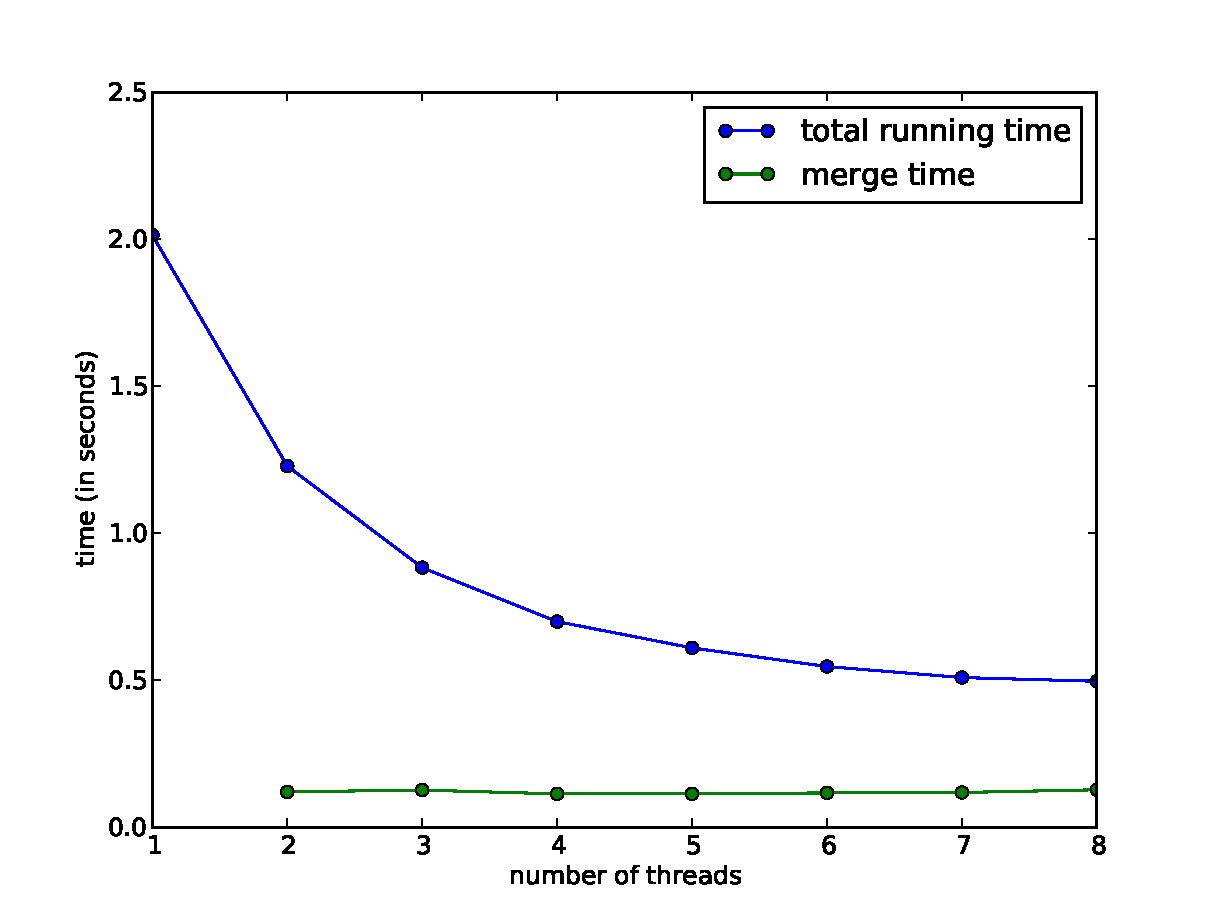
\includegraphics[width=0.5\textwidth]{pcontour.pdf}}
  \quad \subfigure{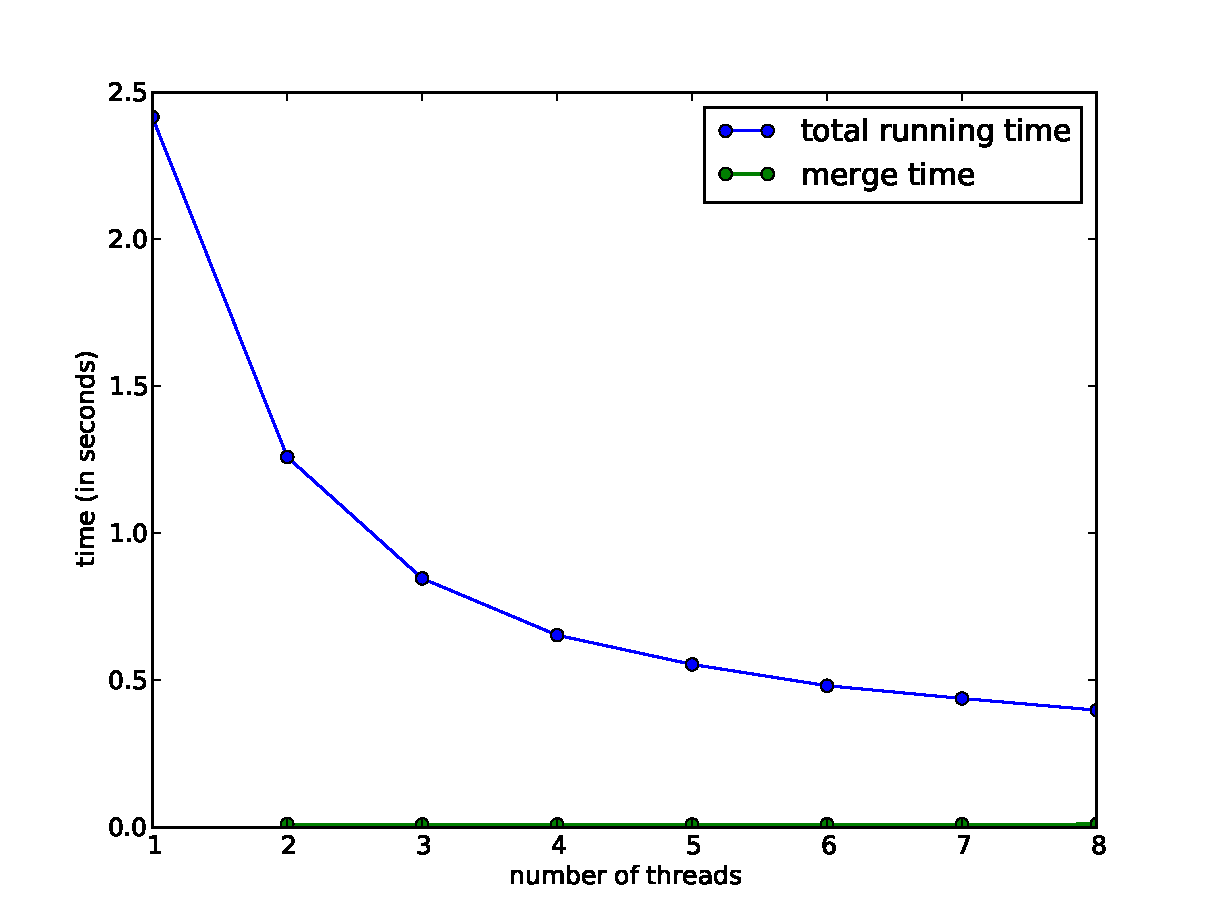
\includegraphics[width=0.5\textwidth]{pcutter.pdf}}
}
\caption{Running time of contouring (left) and cutting (right) as a function of the
  number of parallel threads. Each data measurement is averaged over
  10 runs. The ``merge time'' plot shows the time to merge the
  polygons from all chunks.}
\label{fig:contour}
\end{figure}

\subsubsection*{Code References}
\begin{itemize}
\item Configuration: Release.
\item To generate the plots, run
\begin{enumerate}
\item {\tt python run.py "./pcontour -extent 200 " > pcontour.log}
\item {\tt python run.py "./pcontour -extent 200 -filter cutter" > pcutter.log}
\item {\tt python analyze-pcontour.py pcontour.log}.
\item {\tt python analyze-pcontour.py pcutter.log}.
\end{enumerate}
\end{itemize}

\section{Towards a multithreading framework}

A common parallel algorithm pattern is to divide the data into chunks,
process each chunk in parallel and finally merge the results. We
capture this usage pattern here by adding two extra pipeline passes:
{\tt vtkThreadedCompositeDataPipeline::REQUEST\_DIVIDE} and {\tt
  vtkThreadedCompositeDataPipeline::REQUEST\_MERGE}.  The results in
the previous section are produced using this approach, where image
splitting and surface data merging are handled in the respective
passes.

\section{Comparison with DAX}

We compare the performance of TBB-configured DAX with our
coarse grained approach. We contour two data sets: One has a single
large image; the other is an AMR data set consisting of very small
images. In the first case,the times are similar and, in the second
case, our approach performs better by a small margin.

Figure~\ref{fig:dax-vtk} shows the timing details. We can see that the
two data sets give different scaling behavior. For the super nova data
set, both approaches scale well; for the AMR data set, dax cannot
scale at all, probably due to the fact that the images are too small
that they fall under the minimal TBB grain size.

We should mention that the comparison here is not entirely
apple-to-apple: We use vtkSynchronizedTemplates while DAX has
implemented only the marching cube algorithm; also, our time with no
merging does not concatenate the output chunks, while DAX produces a
single output array. However, considering the similarity of the two
algorithms, we do not expect a more accurate comparison to yield very
different conclusions.


\begin{figure}[H]
\centering \mbox{
  \subfigure{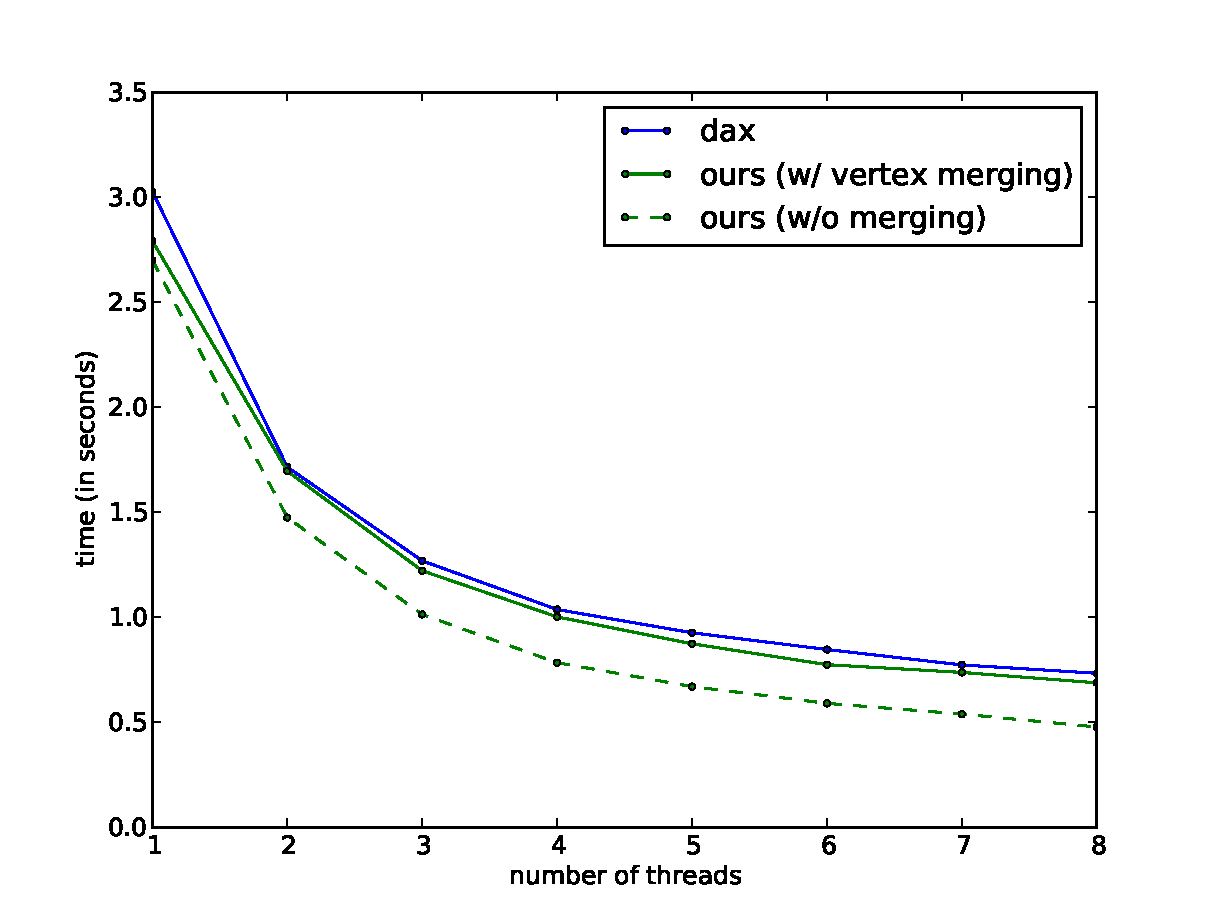
\includegraphics[width=0.5\textwidth]{dax-vtk-supernova.pdf}}
  \quad \subfigure{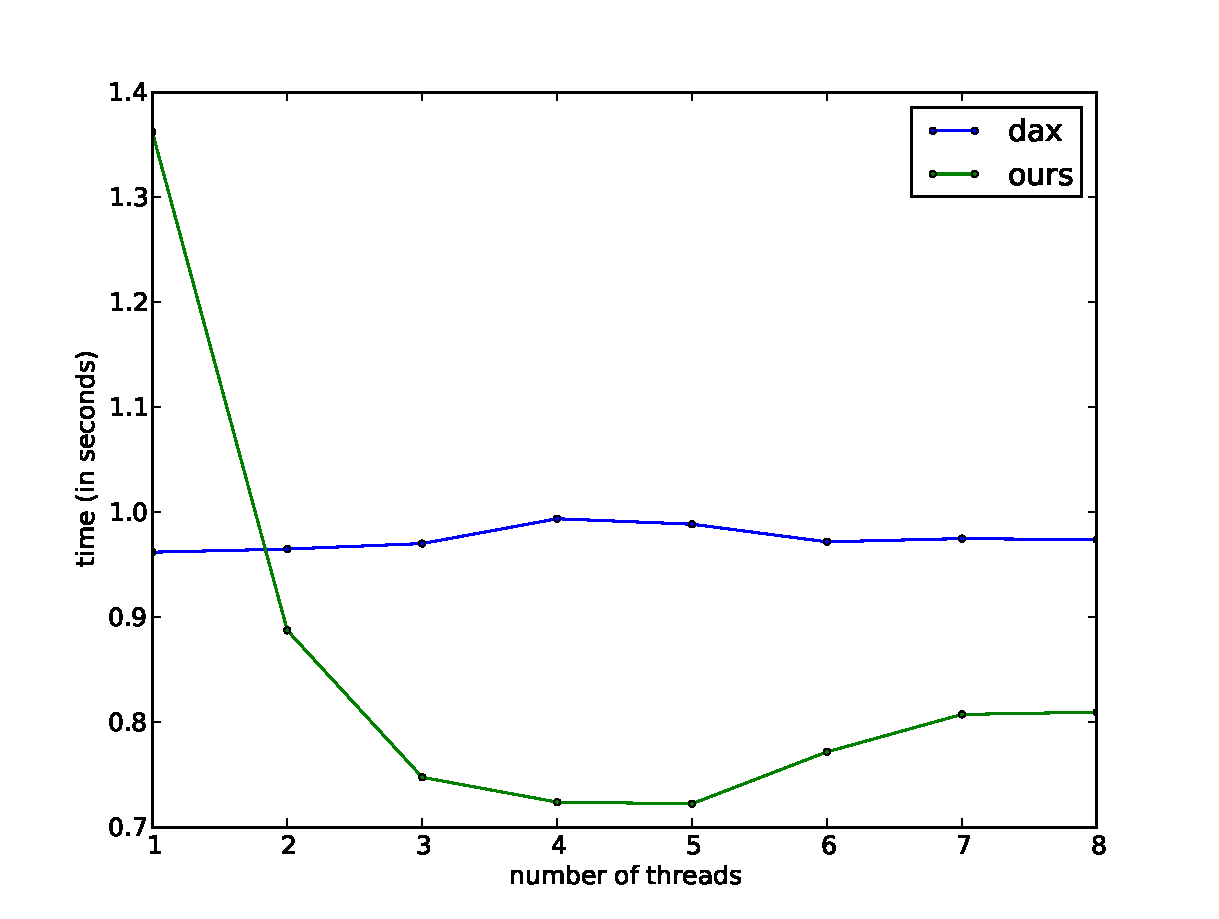
\includegraphics[width=0.5\textwidth]{dax-vtk-smooth.pdf}}
}
\caption{ Contouring time (seconds) plotted against number of
  threads. Left: The input is the ``SuperNova'' datat set---a single
  image of size $432^3$ (provided by Rob Maynard). Right: an AMR data
  set `smooth.flash'', which has around 20 thousands images of
  average size 142 (mostly of dimension $[0..8]^3$). All time
  measurements are averaged over 10 runs.}
\label{fig:dax-vtk}
\end{figure}


\subsubsection*{Code References}
\begin{itemize}
\item The Dax tests are derived from code provided by Robert, in the directory MarchingCubeComparison.
\item The DaxToolKit needs to be modified so that the user can specifiy the maximum number of threads.
\item For the AMR data set, Dax must be configured with {\tt DAX\_USE\_DOUBLE\_PRECISION:BOOL=ON}.
\item For the AMR data set, run {\tt ./contouramr -bigdata} for the dax time and run {\tt ./contouramr -bigdata -vtk}.
\item For the supernova data set, Dax must be configured with {\tt DAX\_USE\_DOUBLE\_PRECISION:BOOL=OFF}
, run ``./marchingCompare -numThreads [number of threads]''.
\end{itemize}

\section{Discussion}

We identify patterns of VTK code that are not thread safe and propose changes.

\begin{itemize}
\item Various subclasses of vtkDataSet have get methods that modify temporary variables. e.g.
{\tt vtkIdType* vtkImageData::GetIncrements()}. The users must call {\tt vtkImageData::GetIncrements(vtkIdType*)}.
\item {\tt vtkAlgorithm::UpdateProgress()} is not thread-safe
\item The debugging configuration {\tt VTK\_DEBUG\_LEAKS:BOOL=OFF} is not thread safe.
\end{itemize}



\section{TBB Notes}

TBB not only calls the {\tt operator()} on a user defined task class,
but also the copy constructor.


\end{document}

scripts:


To do:
- things like InsertNextPoint(),InsertTuple, CopyData() are all very expensive. Should try to see if we can do something like:
- for field in RequiredArrays: do AppendData(field, begin(), end()); parallelizable? even? .
- serious bug in vtkSynchronizedTemplates3D and Cutter3D
-

filters candidate
- point data to cell data
- threshold
- glyph


# comparison with DAX

leo:MarchingCubesComparison-build$ ./marchingCompare
Dax,Serial,3.29341,0
Dax produced 14213868 points 4737956 cells

leo:MarchingCubesComparison-build$ ./marchingCompare
Dax,TBB,1.62712,0
Dax produced 14213868 points 4737956 cells


# on kadoop1

./marchingCompare
Dax,TBB,0.606065,0
Dax produced 14213868 points 4737956 cells
VTK,Serial,2.27258,0
VTK, Serial produced 2376323 points 4737950 cells

leo@kadoop1:~/tbb-build$ ./pcontour --superNova --numThreads 8
8 threads
64 pieces
range: 3.03912e-15 0.114298
Set contour value: 0.07
Merge took 0.208614 seconds
Report output
time: 0.690251 seconds
2376321 points, 4737950 cells 4737950 cell data values



#on my own machine
./contouramr  --bigdata
DAX double Precision
Loaded amr with 97593 blocks
2923626 points, 974542 cells
time: 0.604202 seconds
